\documentclass[11pt,a4paper]{article}

% Packages
\usepackage[margin=2.5cm]{geometry}
\usepackage{microtype}
\usepackage{graphicx}
\usepackage{tikz}
\usetikzlibrary{shapes,arrows.meta,positioning,calc,fit,backgrounds,shadows.blur,decorations.pathmorphing,decorations.pathreplacing}
\usepackage{colortbl}
\usepackage{enumitem}
\usepackage{booktabs}
\usepackage{longtable}
\usepackage{hyperref}
\usepackage{xcolor}
\usepackage{fancyhdr}
\usepackage{titlesec}
\usepackage[most]{tcolorbox}
\usepackage{multicol}
\usepackage{amsmath,amssymb}
\usepackage{multirow}
\usepackage{setspace}
\usepackage{fontawesome5}
\usepackage{listings}

% Spacing
\setlength{\parskip}{3pt plus 1pt minus 1pt}
\setlength{\parindent}{0pt}

% Colors
\definecolor{primary}{HTML}{1A5276}
\definecolor{secondary}{HTML}{2E86C1}
\definecolor{accent}{HTML}{E74C3C}
\definecolor{lightbg}{HTML}{EBF5FB}
\definecolor{defbg}{HTML}{FDF2E9}
\definecolor{greenhl}{HTML}{27AE60}
\definecolor{purplehl}{HTML}{8E44AD}
\definecolor{codebg}{HTML}{F4F6F7}

% Hyperref
\hypersetup{colorlinks=true, linkcolor=primary, urlcolor=secondary, citecolor=primary}

% Code listings style
\lstset{
  backgroundcolor=\color{codebg},
  basicstyle=\ttfamily\small,
  keywordstyle=\color{primary}\bfseries,
  stringstyle=\color{greenhl},
  commentstyle=\color{gray},
  breaklines=true,
  frame=l,
  framerule=2pt,
  rulecolor=\color{secondary!40},
  xleftmargin=8pt,
  framexleftmargin=6pt,
  aboveskip=6pt,
  belowskip=6pt,
  showstringspaces=false,
  language=Python
}

% Header/Footer
\pagestyle{fancy}
\fancyhf{}
\fancyhead[L]{\small\textcolor{primary}{\textbf{Foundations of Data Science, AI, and Emerging Paradigms}}}
\fancyhead[R]{\small\textcolor{primary}{Lecture Handout}}
\fancyfoot[C]{\small\thepage}
\renewcommand{\headrulewidth}{0.5pt}
\renewcommand{\footrulewidth}{0.3pt}

% Section formatting
\titleformat{\section}{\Large\bfseries\color{primary}}{\thesection}{0.6em}{}[\vspace{2pt}\titlerule]
\titleformat{\subsection}{\large\bfseries\color{secondary}}{\thesubsection}{0.5em}{}
\titleformat{\subsubsection}{\normalsize\bfseries\color{primary}}{\thesubsubsection}{0.5em}{}
\titlespacing*{\section}{0pt}{14pt}{8pt}
\titlespacing*{\subsection}{0pt}{10pt}{5pt}

% Custom boxes
\newtcolorbox{definitionbox}[1][]{
  enhanced, breakable,
  colback=defbg, colframe=orange!60!black,
  colbacktitle=orange!70!black, coltitle=white,
  title={\faIcon{book}~#1}, fonttitle=\bfseries,
  boxrule=0pt, leftrule=4pt, arc=2pt,
  shadow={1mm}{-1mm}{0mm}{black!15},
  top=4pt, bottom=4pt, left=8pt, right=8pt
}
\newtcolorbox{conceptbox}[1][]{
  enhanced, breakable,
  colback=lightbg, colframe=secondary,
  colbacktitle=secondary, coltitle=white,
  title={\faIcon{lightbulb}~#1}, fonttitle=\bfseries,
  boxrule=0pt, leftrule=4pt, arc=2pt,
  shadow={1mm}{-1mm}{0mm}{black!15},
  top=4pt, bottom=4pt, left=8pt, right=8pt
}
\newtcolorbox{alertbox}[1][]{
  enhanced, breakable,
  colback=red!4, colframe=accent,
  colbacktitle=accent, coltitle=white,
  title={\faIcon{exclamation-triangle}~#1}, fonttitle=\bfseries,
  boxrule=0pt, leftrule=4pt, arc=2pt,
  shadow={1mm}{-1mm}{0mm}{black!12},
  top=3pt, bottom=3pt, left=8pt, right=8pt
}
\newtcolorbox{examplebox}[1][]{
  enhanced, breakable,
  colback=green!4, colframe=greenhl,
  colbacktitle=greenhl, coltitle=white,
  title={\faIcon{code}~#1}, fonttitle=\bfseries,
  boxrule=0pt, leftrule=4pt, arc=2pt,
  shadow={1mm}{-1mm}{0mm}{black!12},
  top=3pt, bottom=3pt, left=8pt, right=8pt
}

\begin{document}

% Title
\begin{center}
\vspace*{0.5cm}
{\Huge\bfseries\textcolor{primary}{Foundations of Data Science,}}\\[4pt]
{\Huge\bfseries\textcolor{primary}{Artificial Intelligence, and Emerging Paradigms}}\\[16pt]
{\color{secondary}\rule{0.8\textwidth}{1.5pt}}\\[14pt]
{\Large\textsc{Comprehensive Beginner Handout for BSIT Data Science}}\\[8pt]
{\large\textcolor{gray!70!black}{Data Foundations $\bullet$ ML and DL $\bullet$ Generative AI $\bullet$ Agentic AI $\bullet$ Responsible Use}}
\vspace{0.3cm}
\end{center}

\tableofcontents
\newpage

%=============================================================
\section{The Big Picture: Data Science, AI, and Emerging Paradigms}
%=============================================================

\begin{definitionbox}[Data Science]
Data Science is an interdisciplinary field that combines \textbf{statistics, computing, data engineering, machine learning, domain knowledge, and communication} to extract useful insights, build predictive systems, and support better decisions from data.
\end{definitionbox}

\begin{definitionbox}[Artificial Intelligence]
Artificial Intelligence (AI) is the broad field of computer science focused on building systems that can perform tasks that usually require human intelligence, such as reasoning, learning, perception, language understanding, and decision-making.
\end{definitionbox}

\begin{conceptbox}[How These Fields Relate]
Data Science focuses on turning raw data into understanding and action. AI focuses on building intelligent behavior. In practice, the two fields overlap strongly because Data Science often uses AI techniques, while AI systems depend on strong data foundations.
\end{conceptbox}

\subsection{Common Terms in This Handout}

\rowcolors{2}{white}{defbg}
\begin{longtable}{@{}p{3.4cm}p{9.9cm}@{}}
\toprule
\rowcolor{primary!15}
\textbf{Field or Term} & \textbf{Main Focus} \\
\midrule
\endhead
Data Science & End-to-end process of collecting, cleaning, analyzing, modeling, and using data \\
\addlinespace
Data Mining & Discovering patterns and relationships from data \\
\addlinespace
Machine Learning & Learning patterns from data to make predictions or decisions \\
\addlinespace
Deep Learning & Using multi-layer neural networks for complex learning tasks \\
\addlinespace
Generative AI & Creating new content such as text, images, code, or audio \\
\addlinespace
Agentic AI & Building goal-directed systems that can reason, plan, and act \\
\bottomrule
\end{longtable}

\subsection{AI as the Umbrella Field}

\begin{center}
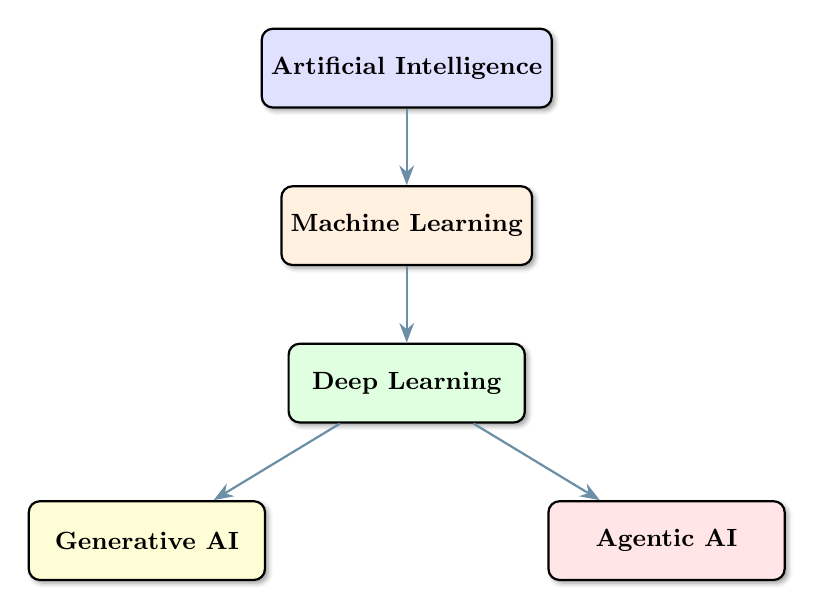
\begin{tikzpicture}[
  box/.style={rectangle, draw, thick, fill=#1, minimum width=3.0cm, minimum height=1.0cm, align=center, font=\small\bfseries, rounded corners=4pt,
    blur shadow={shadow blur steps=4, shadow xshift=0.4mm, shadow yshift=-0.4mm}},
  arr/.style={-{Stealth[length=2.5mm]}, thick, primary!65}
]
  \node[box=blue!12] (ai) at (0,0) {Artificial Intelligence};
  \node[box=orange!12] (ml) at (0,-2.0) {Machine Learning};
  \node[box=green!12] (dl) at (0,-4.0) {Deep Learning};
  \node[box=yellow!16] (gen) at (-3.3,-6.0) {Generative AI};
  \node[box=red!10] (agent) at (3.3,-6.0) {Agentic AI};

  \draw[arr] (ai) -- (ml);
  \draw[arr] (ml) -- (dl);
  \draw[arr] (dl) -- (gen);
  \draw[arr] (dl) -- (agent);
\end{tikzpicture}
\end{center}

\begin{itemize}[leftmargin=*]
  \item \textbf{Machine Learning} is a major subfield of AI.
  \item \textbf{Deep Learning} is a specialized branch of machine learning.
  \item \textbf{Generative AI} and \textbf{Agentic AI} are important emerging paradigms built on modern AI and deep learning methods.
\end{itemize}

%=============================================================
\section{Foundations of Data Science}
%=============================================================

\subsection{Why Data Science Matters}

\begin{itemize}[leftmargin=*]
  \item It helps organizations and researchers turn raw data into evidence.
  \item It supports descriptive, predictive, and prescriptive decision-making.
  \item It combines technical methods with domain understanding and communication.
  \item It provides the full pipeline from data collection to deployment and monitoring.
\end{itemize}

\subsection{Data Mining vs. Data Science}

\begin{center}
\begin{tabular}{@{}p{4.0cm}p{4.2cm}p{4.6cm}@{}}
\toprule
\textbf{Aspect} & \textbf{Data Mining} & \textbf{Data Science} \\
\midrule
Main goal & Discover hidden patterns & Deliver end-to-end value from data \\
Main focus & Pattern discovery and knowledge extraction & Full lifecycle including modeling, deployment, and decision support \\
Typical scope & Analysis-centered & Analysis plus engineering, automation, and communication \\
Relationship & Important component & Broader field that includes data mining \\
\bottomrule
\end{tabular}
\end{center}

\begin{conceptbox}[Key Point]
Data mining is not separate from Data Science. It is one important part of the broader Data Science lifecycle.
\end{conceptbox}

\subsection{The Extended Data Science Lifecycle}

\begin{center}
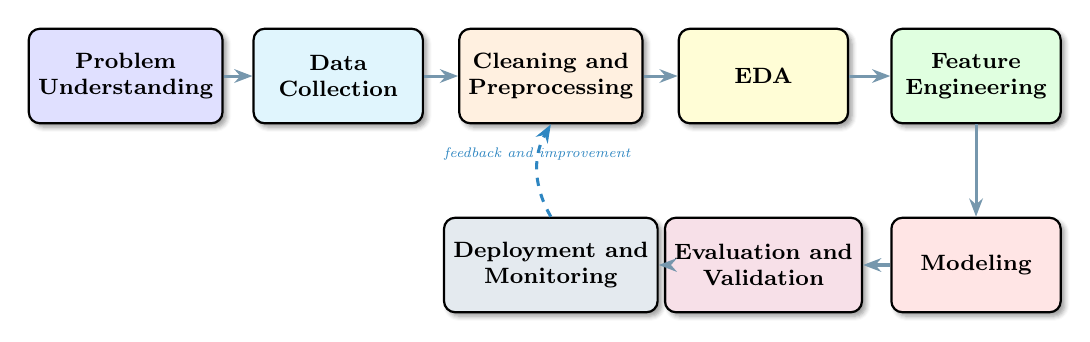
\begin{tikzpicture}[
  step/.style={rectangle, draw, thick, fill=#1, minimum width=2.15cm, minimum height=1.2cm, align=center, font=\footnotesize\bfseries, rounded corners=4pt,
    blur shadow={shadow blur steps=5, shadow xshift=0.5mm, shadow yshift=-0.5mm}},
  arr/.style={-{Stealth[length=2.3mm]}, very thick, primary!60, line width=1.1pt}
]
  \node[step=blue!12]   (s1) at (0,0)    {Problem\\Understanding};
  \node[step=cyan!12]   (s2) at (2.7,0)  {Data\\Collection};
  \node[step=orange!12] (s3) at (5.4,0)  {Cleaning and\\Preprocessing};
  \node[step=yellow!16] (s4) at (8.1,0)  {EDA};
  \node[step=green!12]  (s5) at (10.8,0) {Feature\\Engineering};
  \node[step=red!10]    (s6) at (10.8,-2.4) {Modeling};
  \node[step=purple!12] (s7) at (8.1,-2.4) {Evaluation and\\Validation};
  \node[step=primary!12](s8) at (5.4,-2.4) {Deployment and\\Monitoring};

  \draw[arr] (s1) -- (s2);
  \draw[arr] (s2) -- (s3);
  \draw[arr] (s3) -- (s4);
  \draw[arr] (s4) -- (s5);
  \draw[arr] (s5) -- (s6);
  \draw[arr] (s6) -- (s7);
  \draw[arr] (s7) -- (s8);
  \draw[arr, dashed, secondary] (s8.north) to[bend left=30] node[above, font=\tiny\itshape, secondary] {feedback and improvement} (s3.south);
\end{tikzpicture}
\end{center}

\begin{enumerate}[leftmargin=*]
  \item \textbf{Problem or business understanding:} Define the question and the goal.
  \item \textbf{Data collection:} Gather raw data from relevant sources.
  \item \textbf{Data cleaning and preprocessing:} Handle missing values, duplicates, errors, and inconsistent formats.
  \item \textbf{Exploratory Data Analysis (EDA):} Summarize, visualize, and understand the data.
  \item \textbf{Feature engineering:} Transform data into better inputs for modeling.
  \item \textbf{Modeling:} Apply machine learning or deep learning methods.
  \item \textbf{Evaluation and validation:} Test whether the solution works reliably.
  \item \textbf{Deployment and monitoring:} Put the solution into use and track its performance over time.
\end{enumerate}

\begin{conceptbox}[Why the Lifecycle Matters]
The lifecycle shows that Data Science is not just about building a model. It is about creating a complete system that solves a real problem and remains useful after deployment.
\end{conceptbox}

%=============================================================
\section{Core Data Foundations}
%=============================================================

\subsection{Dataset, Subject, and Observation}

\begin{definitionbox}[Dataset]
A dataset is a structured, semi-structured, or unstructured collection of observations that represents real-world entities, events, or processes.
\end{definitionbox}

\begin{itemize}[leftmargin=*]
  \item \textbf{Subject or entity of analysis:} What the dataset is about.
  \item \textbf{Observation or instance:} One row, record, case, or sample in the dataset.
\end{itemize}

Examples:
\begin{itemize}[leftmargin=*]
  \item Students in an educational analytics dataset
  \item Patients in a healthcare dataset
  \item Customers in a business dataset
\end{itemize}

\begin{alertbox}[Important Modeling Principle]
Correctly identifying the subject and observation unit is essential. If the unit of analysis is wrong, the model and conclusions may also be wrong.
\end{alertbox}

\subsection{Structure of Data}

\rowcolors{2}{white}{defbg}
\begin{longtable}{@{}p{3.0cm}p{3.8cm}p{6.7cm}@{}}
\toprule
\rowcolor{primary!15}
\textbf{Data Form} & \textbf{Main Characteristic} & \textbf{Examples} \\
\midrule
\endhead
Structured data & Fixed rows and columns & CSV files, Excel sheets, relational databases \\
\addlinespace
Semi-structured data & Flexible schema, tagged or nested format & JSON, XML, logs, API responses \\
\addlinespace
Unstructured data & No fixed schema & Text, images, audio, video \\
\bottomrule
\end{longtable}

\begin{conceptbox}[Modern AI and Data]
Classical machine learning often works well on structured data, while modern AI and deep learning are especially important for semi-structured and unstructured data such as text, images, and audio.
\end{conceptbox}

\subsection{Features and Target Variables}

\begin{definitionbox}[Features]
Features are the measurable characteristics or attributes that describe an entity. They are usually the input variables used by a model.
\end{definitionbox}

\begin{definitionbox}[Target Variable or Label]
The target variable is the outcome that we want to predict or explain.
\end{definitionbox}

Example for a student dataset:
\begin{itemize}[leftmargin=*]
  \item \textbf{Features:} Attendance rate, prior GPA, LMS activity time
  \item \textbf{Target:} Final GPA, pass or fail, dropout risk
\end{itemize}

\begin{conceptbox}[Feature Engineering]
Feature engineering is the process of selecting, transforming, or creating better features so that a model can learn more effectively.
\end{conceptbox}

\subsection{Measurement Scales and Data Types}

\rowcolors{2}{white}{defbg}
\begin{longtable}{@{}p{3.0cm}p{3.6cm}p{6.9cm}@{}}
\toprule
\rowcolor{primary!15}
\textbf{Type} & \textbf{Meaning} & \textbf{Why It Matters} \\
\midrule
\endhead
Nominal & Unordered categories & Requires encoding because categories have no numeric order \\
\addlinespace
Ordinal & Ordered categories & Order matters, but numerical distance may not \\
\addlinespace
Discrete numerical & Countable values & Common in counting tasks and event-based data \\
\addlinespace
Continuous numerical & Real-valued measurements & Important for regression, scaling, and distance-based methods \\
\bottomrule
\end{longtable}

\begin{itemize}[leftmargin=*]
  \item Understanding data types helps with algorithm selection.
  \item It also affects encoding, distance computation, and data preprocessing.
\end{itemize}

\subsection{Labeled, Unlabeled, and Semi-Supervised Data}

\begin{itemize}[leftmargin=*]
  \item \textbf{Labeled data:} Features are paired with a known output. Used in supervised learning.
  \item \textbf{Unlabeled data:} No target variable is available. Used in unsupervised learning.
  \item \textbf{Semi-supervised learning:} Combines a small amount of labeled data with a larger amount of unlabeled data.
\end{itemize}

\subsection{Primary and Secondary Data Sources}

\begin{itemize}[leftmargin=*]
  \item \textbf{Primary data:} Collected directly for the current purpose. Usually offers more control, but takes more time and cost.
  \item \textbf{Secondary data:} Already exists from previous studies, public repositories, organizations, or systems.
\end{itemize}

\subsection{Other Essential Beginner Concepts}

\begin{itemize}[leftmargin=*]
  \item \textbf{Missing values:} Data fields that are empty or unknown.
  \item \textbf{Duplicates:} Repeated records that may distort analysis.
  \item \textbf{Outliers:} Extreme values that may be unusual or informative.
  \item \textbf{Train, validation, and test sets:} Separate data portions used to train, tune, and evaluate a model fairly.
\end{itemize}

%=============================================================
\section{Levels of Analytics in Data Science}
%=============================================================

\rowcolors{2}{white}{defbg}
\begin{longtable}{@{}p{3.1cm}p{3.8cm}p{5.2cm}@{}}
\toprule
\rowcolor{primary!15}
\textbf{Analytics Level} & \textbf{Guiding Question} & \textbf{Typical Methods} \\
\midrule
\endhead
Descriptive / exploratory & What happened? & Summary statistics, tables, charts, EDA \\
\addlinespace
Diagnostic & Why did it happen? & Root-cause analysis, comparisons, drill-down analysis \\
\addlinespace
Predictive & What will happen? & Classification, regression, forecasting, ML and DL \\
\addlinespace
Prescriptive & What should we do? & Optimization, recommendation, simulation, decision support \\
\bottomrule
\end{longtable}

\begin{conceptbox}[Analytics Maturity]
As we move from descriptive to prescriptive analytics, the focus shifts from understanding the past to guiding future decisions and actions.
\end{conceptbox}

%=============================================================
\section{Machine Learning, Deep Learning, and Data Mining}
%=============================================================

\subsection{Machine Learning}

\begin{definitionbox}[Machine Learning]
Machine Learning (ML) enables systems to learn patterns from data and make predictions or decisions without being explicitly programmed with fixed rules for every situation.
\end{definitionbox}

Common machine learning tasks:
\begin{itemize}[leftmargin=*]
  \item \textbf{Classification:} Predicting categories such as pass or fail, spam or not spam.
  \item \textbf{Regression:} Predicting numerical values such as income, GPA, or price.
  \item \textbf{Clustering:} Grouping similar items together when labels are not available.
\end{itemize}

\subsection{Deep Learning}

\begin{definitionbox}[Deep Learning]
Deep Learning is a specialized branch of machine learning that uses neural networks with many layers to learn complex and hierarchical patterns from large datasets.
\end{definitionbox}

Deep learning powers:
\begin{itemize}[leftmargin=*]
  \item Large Language Models (LLMs)
  \item Image generation systems
  \item Speech recognition systems
  \item Modern generative models
\end{itemize}

\begin{conceptbox}[Simple Comparison]
Classical machine learning often depends more heavily on manual feature engineering, while deep learning can automatically learn complex representations from raw or minimally processed data.
\end{conceptbox}

\subsection{How Data Mining Fits Here}

\begin{definitionbox}[Data Mining]
Data Mining focuses on discovering meaningful patterns, trends, correlations, or structures from large datasets using statistical and machine learning techniques.
\end{definitionbox}

\begin{itemize}[leftmargin=*]
  \item Its main emphasis is \textbf{pattern discovery}, \textbf{knowledge extraction}, and \textbf{interpretation}.
  \item It is highly relevant during EDA and pattern analysis within the Data Science workflow.
\end{itemize}

%=============================================================
\section{Generative AI}
%=============================================================

\begin{definitionbox}[Generative AI]
Generative AI refers to models that learn the underlying patterns or probability distribution of data and then generate new outputs that resemble the training data, such as text, images, code, audio, or video.
\end{definitionbox}

\begin{conceptbox}[Generative vs Predictive]
Predictive systems estimate labels or values. Generative systems create new content.
\end{conceptbox}

\subsection{Core Characteristics of Generative AI}

\begin{itemize}[leftmargin=*]
  \item Learns data distributions and patterns
  \item Produces novel outputs rather than only class labels
  \item Often behaves probabilistically, meaning outputs can vary
  \item Usually depends on very large-scale datasets and deep learning models
\end{itemize}

\subsection{Common Generative Model Families}

\rowcolors{2}{white}{defbg}
\begin{longtable}{@{}p{3.1cm}p{3.6cm}p{6.3cm}@{}}
\toprule
\rowcolor{primary!15}
\textbf{Model Family} & \textbf{Typical Output} & \textbf{Key Idea} \\
\midrule
\endhead
Autoregressive models & Text, code, sequences & Generate outputs step by step, often token by token \\
\addlinespace
Variational Autoencoders (VAEs) & Synthetic samples, compressed representations & Learn a latent representation and generate from it \\
\addlinespace
Generative Adversarial Networks (GANs) & Synthetic images and samples & A generator and discriminator learn through competition \\
\addlinespace
Diffusion models & Images, audio, video & Start from noise and refine it into meaningful output \\
\bottomrule
\end{longtable}

\subsection{Important Beginner Terms for Generative AI}

\begin{itemize}[leftmargin=*]
  \item \textbf{Prompt:} The instruction given to the model.
  \item \textbf{Token:} A small unit of text processed by the model.
  \item \textbf{Context window:} The amount of information the model can consider at one time.
  \item \textbf{Inference:} The stage when the trained model generates an answer for a new input.
\end{itemize}

\subsection{GitHub Copilot as Generative AI in Practice}

\begin{definitionbox}[GitHub Copilot]
GitHub Copilot is an AI-powered code generation assistant integrated into development environments such as VS Code. It uses deep learning and large language models to help users write, explain, and improve code.
\end{definitionbox}

For Data Science work, GitHub Copilot can:
\begin{itemize}[leftmargin=*]
  \item Suggest data preprocessing code
  \item Help write feature engineering steps
  \item Generate visualization scripts
  \item Assist with model implementation
  \item Explain functions and error messages
  \item Speed up experimentation and prototyping
\end{itemize}

\subsection{Common Copilot Modes in Modern Editors}

\rowcolors{2}{white}{defbg}
\begin{longtable}{@{}p{2.7cm}p{3.8cm}p{5.9cm}@{}}
\toprule
\rowcolor{primary!15}
\textbf{Mode} & \textbf{What It Does} & \textbf{Typical Student Use} \\
\midrule
\endhead
Ask mode & Explains concepts, code, or errors & Learn syntax, understand models, ask questions \\
\addlinespace
Edit mode & Applies requested code or text changes & Refactor notebooks, adjust scripts, rewrite blocks \\
\addlinespace
Agent mode & Works through multi-step tasks using tools and repo context & Search files, update several places, validate changes \\
\bottomrule
\end{longtable}

\begin{alertbox}[Important Reminder About Copilot]
GitHub Copilot suggestions must always be reviewed, tested, and understood. Generated code can still contain errors, bias, or insecure practices.
\end{alertbox}

%=============================================================
\section{Agentic AI}
%=============================================================

\begin{definitionbox}[Agentic AI]
Agentic AI refers to autonomous or semi-autonomous AI systems that can perceive inputs, reason about goals, plan actions, execute decisions, and adapt over time.
\end{definitionbox}

\subsection{Core Components of an AI Agent}

\begin{itemize}[leftmargin=*]
  \item \textbf{Perception:} Observing input, context, or environment
  \item \textbf{Reasoning:} Interpreting the situation and choosing what makes sense
  \item \textbf{Planning:} Sequencing steps toward a goal
  \item \textbf{Action:} Executing tasks through tools, APIs, or generated outputs
  \item \textbf{Memory:} Keeping useful context for future steps
\end{itemize}

\subsection{Agentic Feedback Loop}

\begin{center}
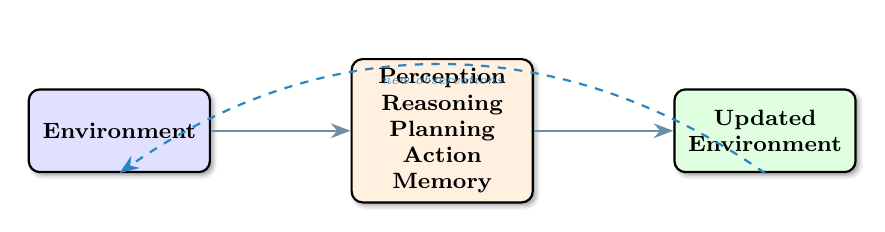
\begin{tikzpicture}[
  step/.style={rectangle, draw, thick, fill=#1, minimum width=2.3cm, minimum height=1.05cm, align=center, font=\footnotesize\bfseries, rounded corners=4pt,
    blur shadow={shadow blur steps=4, shadow xshift=0.4mm, shadow yshift=-0.4mm}},
  arr/.style={-{Stealth[length=2.5mm]}, thick, primary!65}
]
  \node[step=blue!12] (env1) at (0,0) {Environment};
  \node[step=orange!12] (agent) at (4.1,0) {Perception\\Reasoning\\Planning\\Action\\Memory};
  \node[step=green!12] (env2) at (8.2,0) {Updated\\Environment};

  \draw[arr] (env1) -- (agent);
  \draw[arr] (agent) -- (env2);
  \draw[arr, dashed, secondary] (env2.south) to[bend right=35] node[below, font=\tiny\itshape, secondary] {new observations} (env1.south);
\end{tikzpicture}
\end{center}

\subsection{Applications of Agentic AI}

\begin{itemize}[leftmargin=*]
  \item Autonomous research assistants
  \item Intelligent tutoring systems
  \item Workflow automation agents
  \item Academic advising systems
  \item Decision-support systems
\end{itemize}

\begin{conceptbox}[Relationship to Generative AI]
Agentic AI often uses a generative model such as an LLM as its reasoning engine, but extends it with planning, memory, tools, and action loops.
\end{conceptbox}

%=============================================================
\section{Generative AI vs. Agentic AI}
%=============================================================

\begin{center}
\begin{tabular}{@{}p{2.8cm}p{4.2cm}p{4.2cm}@{}}
\toprule
\textbf{Aspect} & \textbf{Generative AI} & \textbf{Agentic AI} \\
\midrule
Primary focus & Content generation & Goal-driven action \\
Core capability & Generate text, images, code, or audio & Decide, plan, and act \\
Autonomy & Often limited & Higher and more persistent \\
Interaction style & Prompt-based & Environment-based or tool-based \\
Memory & Often short-term & Often persistent or state-aware \\
Typical output & Content & Actions, plans, decisions, and content \\
\bottomrule
\end{tabular}
\end{center}

\begin{conceptbox}[Integration Principle]
Generative AI often acts as the cognitive engine inside an agentic system, while agentic AI adds planning logic, tools, memory, and goal management around that engine.
\end{conceptbox}

%=============================================================
\section{Architectural Perspectives}
%=============================================================

\subsection{Generative Model Flow}

\begin{center}
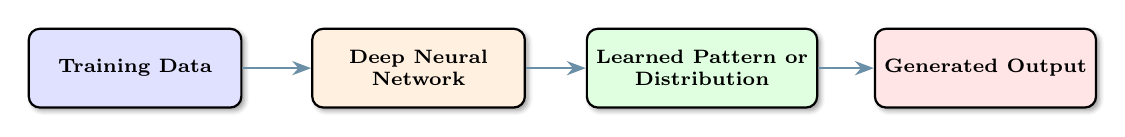
\begin{tikzpicture}[
  box/.style={rectangle, draw, thick, fill=#1, minimum width=2.7cm, minimum height=1.0cm, align=center, font=\scriptsize\bfseries, rounded corners=4pt,
    blur shadow={shadow blur steps=4, shadow xshift=0.4mm, shadow yshift=-0.4mm}},
  arr/.style={-{Stealth[length=2.4mm]}, thick, primary!65}
]
  \node[box=blue!12] (d1) at (0,0) {Training Data};
  \node[box=orange!12] (d2) at (3.6,0) {Deep Neural\\Network};
  \node[box=green!12] (d3) at (7.2,0) {Learned Pattern or\\Distribution};
  \node[box=red!10] (d4) at (10.8,0) {Generated Output};

  \draw[arr] (d1) -- (d2);
  \draw[arr] (d2) -- (d3);
  \draw[arr] (d3) -- (d4);
\end{tikzpicture}
\end{center}

\subsection{Combined Agentic Architecture}

\begin{center}
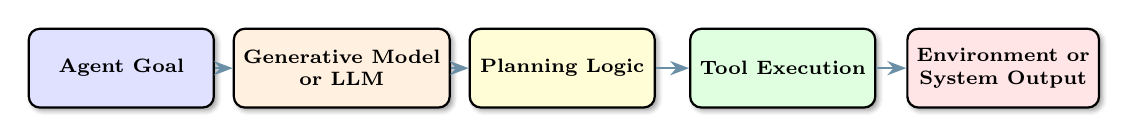
\begin{tikzpicture}[
  box/.style={rectangle, draw, thick, fill=#1, minimum width=2.35cm, minimum height=1.0cm, align=center, font=\scriptsize\bfseries, rounded corners=4pt,
    blur shadow={shadow blur steps=4, shadow xshift=0.4mm, shadow yshift=-0.4mm}},
  arr/.style={-{Stealth[length=2.4mm]}, thick, primary!65}
]
  \node[box=blue!12] (a1) at (0,0) {Agent Goal};
  \node[box=orange!12] (a2) at (2.8,0) {Generative Model\\or LLM};
  \node[box=yellow!16] (a3) at (5.6,0) {Planning Logic};
  \node[box=green!12] (a4) at (8.4,0) {Tool Execution};
  \node[box=red!10] (a5) at (11.2,0) {Environment or\\System Output};

  \draw[arr] (a1) -- (a2);
  \draw[arr] (a2) -- (a3);
  \draw[arr] (a3) -- (a4);
  \draw[arr] (a4) -- (a5);
\end{tikzpicture}
\end{center}

\begin{conceptbox}[Future Direction]
Modern intelligent systems increasingly combine strong data foundations, predictive modeling, generative capabilities, and agentic behavior into practical, scalable, and domain-aware solutions.
\end{conceptbox}

%=============================================================
\section{Ethical and Practical Considerations}
%=============================================================

\rowcolors{2}{white}{defbg}
\begin{longtable}{@{}p{3.2cm}p{4.1cm}p{5.9cm}@{}}
\toprule
\rowcolor{primary!15}
\textbf{Issue} & \textbf{What It Means} & \textbf{Why It Matters} \\
\midrule
\endhead
Bias and fairness & Outputs may reflect unfair patterns in data & Can harm people and reduce trust \\
\addlinespace
Hallucination and reliability & Models may produce believable but false content & Can mislead decisions and reports \\
\addlinespace
Privacy and security & Sensitive data may be exposed or mishandled & Important in education, health, and business contexts \\
\addlinespace
Over-reliance on AI & Users may accept outputs without review & Human understanding and validation remain essential \\
\addlinespace
Responsible deployment & Systems need limits, testing, and governance & Important for education, research, and real-world use \\
\bottomrule
\end{longtable}

\begin{alertbox}[Educational Responsibility]
In BSIT and Data Science courses, AI tools can support learning, but they should not replace understanding. Students are responsible for reviewing generated code, verifying answers, and explaining their own work.
\end{alertbox}

\begin{conceptbox}[Human-in-the-Loop]
Human-in-the-loop means that people remain involved in checking, approving, or correcting AI decisions, especially when the results matter for grades, academic work, policy, security, or public use.
\end{conceptbox}

%=============================================================
\section{Integrated Summary}
%=============================================================

\begin{itemize}[leftmargin=*]
  \item Data Science provides the structured lifecycle for transforming raw data into useful insights and deployed systems.
  \item Data Mining focuses on discovering patterns and is one component within the broader Data Science workflow.
  \item Machine Learning and Deep Learning power predictive and intelligent systems.
  \item Generative AI creates new content such as text, images, and code, with GitHub Copilot as a practical coding example.
  \item Agentic AI builds goal-directed systems that perceive, reason, plan, act, and adapt.
  \item The future of intelligent systems lies in combining strong data foundations, robust models, generative capabilities, and agentic architectures in responsible ways.
\end{itemize}

%=============================================================
\section{Review Questions}
%=============================================================

\begin{enumerate}[leftmargin=*]
  \item What is the difference between Data Science and Data Mining?
  \item Why is Artificial Intelligence described as an umbrella field?
  \item What are the common tasks in machine learning?
  \item How does deep learning differ from classical machine learning?
  \item Why is it important to identify the subject and observation unit correctly?
  \item What is the difference between structured, semi-structured, and unstructured data?
  \item How do descriptive, predictive, and prescriptive analytics differ?
  \item What makes Generative AI different from predictive AI?
  \item How is GitHub Copilot an example of Generative AI in practice?
  \item What are the core components of an AI agent?
  \item How does Agentic AI differ from Generative AI?
  \item Why are ethics, privacy, and human review important in Data Science and AI systems?
\end{enumerate}

\end{document}